\subsection*{Model}
The function described in this problem is the following
\begin{equation*}
    \begin{aligned}
    & F(\mathbf{x}) = \frac{1}{2} \sum_{k=1}^{n} f_k^2(x) \\
    & f_k(\mathbf{x}) = 10 \left(x_k^2 - x_{k+1}\right), \quad  & \mod (k,2) = 1\\   
    & f_k(\mathbf{x}) = x_{k-1} -1, \quad & \mod(k,2) = 0
    \end{aligned}
\end{equation*}
where $n$ denotes the dimensionality of the input vector $\mathbf{x}$. As convention, we set $x_{n+1} = x_1$ when it is necessary, that is when the dimensionality $n$ is an odd number.
\\ The starting point for the minimization is the vector $\mathbf{x}_0 = [-1.2, 1, -1.2, 1, \ldots]$.

In order to compute the derivatives of this problem we have to consider separately the cases when $n$ is even or odd. In the first case, the gradient of the function is given by
\begin{align*}
    &\frac{\partial F}{\partial x_k} (\mathbf{x}) = \frac{\partial}{\partial x_k} \left[\frac{1}{2} f_{k-1}^2(\mathbf{x})\right] = - 100 (x_{k-1}^2 - x_k) \quad & \mod(k,2) = 0 \\
    & \frac{\partial F}{\partial x_k} (\mathbf{x}) = \frac{\partial}{\partial x_k} \left[\frac{1}{2} f_{k}^2(\mathbf{x}) + \frac{1}{2} f_{k+1}^2(\mathbf{x})\right] = 200x_k (x_k^2 - x_{k+1}) + (x_k -1)\quad & \mod(k,2) = 1
\end{align*}

If the dimensionality $n$ is odd, the only change is in the first component of the gradient, which becomes
$$ \frac{\partial F}{\partial x_1} (\mathbf{x})  = \frac{\partial}{\partial x_k} \left[\frac{1}{2} f_{k}^2(\mathbf{x}) + \frac{1}{2} f_{k+1}^2(\mathbf{x}) + \frac{1}{2}f_n^2(\mathbf{x}) \right] = 200x_1 (x_1^2 - x_{2}) + (x_1 -1)  - 100(x_n^2 - x_1)$$

Looking at the structure of the problem we are considering, it is obvious that the Hessian matrix is a sparse matrix whose particular structure depends again on whether $n$ is even or odd. In the first case, the Hessian is a block trigonal matrix with the following non-zero terms
\begin{align*}
    \frac{\partial^2 F}{\partial x_k^2} (\mathbf{x}) &= 100, & \frac{\partial^2 F}{\partial x_k \partial x_{k+1}} (\mathbf{x}) &= 0, & \frac{\partial^2 F}{\partial x_k \partial x_{k-1}} (\mathbf{x}) &= -200x_{k-1} & \mod(k,2) &= 0 \\
    \frac{\partial^2 F}{\partial x_k^2} (\mathbf{x}) &= 600x_k^2 - 200x_{k+1} + 1, & \frac{\partial^2 F}{\partial x_k \partial x_{k+1}} (\mathbf{x}) &= -200x_k, & \frac{\partial^2 F}{\partial x_k \partial x_{k-1}} (\mathbf{x}) &= 0 & \mod(k,2) &= 1 \\
\end{align*}

If $n$ is odd, there are two changes in the Hessian matrix: the derivative $\frac{\partial^2 F}{\partial x_1^2} (\mathbf{x}) $ is affected by the presence of $x_1$ in the term $f_n()$ and the external diagonals are not zero anymore. We report the terms of the Hessian matrix that differs from the previous case
\begin{align*}
    \frac{\partial^2 F}{\partial x_1^2}  (\mathbf{x}) &= 600x_k^2 - 200x_{k+1} + 101 \\
    \frac{\partial^2 F}{\partial x_n \partial x_1} (\mathbf{x}) &= \frac{\partial^2 F}{\partial x_1 \partial x_n} (\mathbf{x}) = -200x_n
\end{align*}

By analyzing the derivatives of the problem, we can deduce that the gradient of the function is nullified by the vector composed of ones which also nullifies the value of $F(\mathbf{x})$. 
As a matter of fact, we can notice that the terms $f_k()$ for an odd value of $k$ are nullified only when $x_{k - 1} = 1$, while the terms $f_k()$ for an even value of $k$ are nullified when $1 = x_k^2 = x_{k+1}$. This leads to the conclusion that the function $F(\mathbf{x})$ assumes its lower value, in other words is nullified, when for the vector $\mathbf{x} = \mathbbm{1}$, which, indeed, is a global minimum.
\\ To better understand the behavior of the function $F(\mathbf{x})$ in the neighborhood of the minimizer we have found, we now report a plot of the function in 2D for $n = 2$. 
\begin{figure}[H]
    \centering
    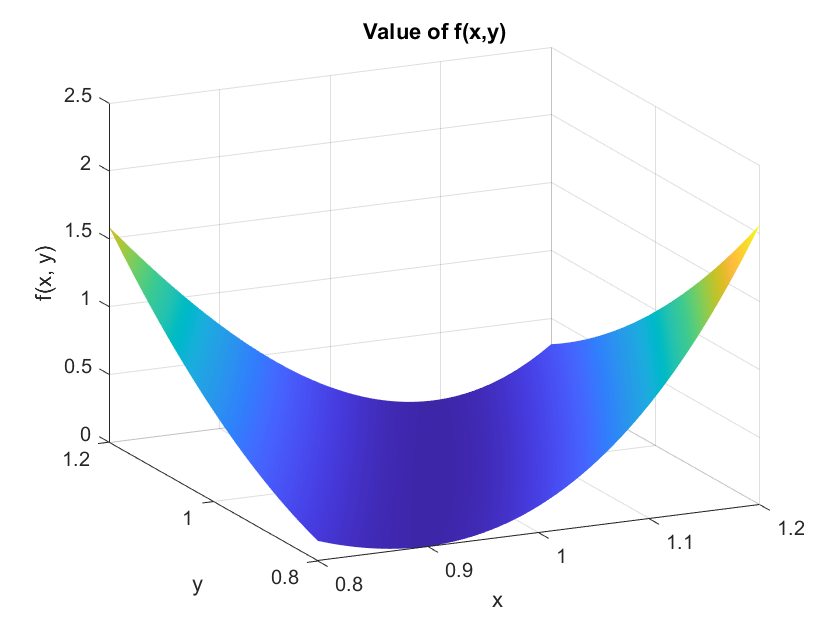
\includegraphics[width=0.5\textwidth]{img/pb25_fig.png}
    \caption{2D plot of the function $F(x_1, x_2)$.}
\end{figure}
From the plot, we can notice that the function is almost flat near the minimum; this may affect the performances of the algorithms implemented because flat regions may be the cause of slow convergence or even stagnation for optimization solvers. 

 
\medskip
\subsection*{Nealder Mead Method}
We run the experiments with Nealder Mea method using the following parameters:
\begin{equation*}
    \text{reflection } \rho = 1 \quad
    \text{expansion } \chi = 2 \quad
    \text{contraction } \gamma = 0.5 \quad
    \text{shrinking } \sigma = 0.5
\end{equation*}
and fixing the tolerance to $10^{-4}$.
\\ For each dimensionality, $n \in \{10; 25; 50\}$, $11$ experiments have been run, each of them starting from a different initial point; in particular, one of these initial point is the one declared at the beginning, the others have been obtained as perturbations of the first initial guess.

The table $\eqref{SX25}$ shows some general results of these experiments, such as the value of the minimum point found, the average number of iterations used by the method, the average time of execution, the number of failures declared for each dimensionality and the average rate of convergence.
\begin{figure*}[htbp]
    \centering
    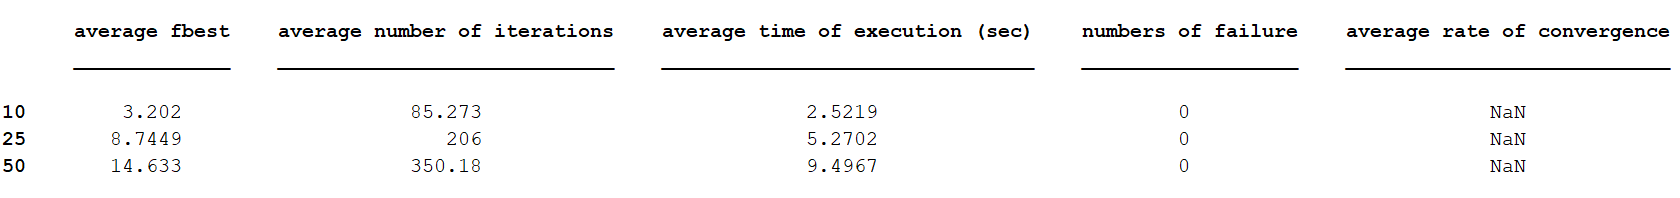
\includegraphics[width = 0.9\textwidth]{img/pb25_SX_table.png}
    \caption{Results obtained by running the simplex method on the problem $25$.}
    \label{SX25}
\end{figure*}

Looking at the table, it is clear that even if the method satisfies the stopping criterion for all dimensionalities it does not reach the point we declared be a global minimum, actually the minimum value the algorithm finds increases with the dimensionality.
We are not too surprised by the poor performance of the simplex method because the algorithm solely relies on function evaluation and does not take advantage of the information contained in the derivatives of the objective function and thus it is possible that it got stuck in the flat zone of the function.

The column that should contain the average rate of convergence is filled with \verb+NaN+ values. This occurs because the best value found by the method remains almost stationary in the last few iterations, usually during the shrinking phase. As a result, in the formula $\eqref{definizione_roc}$, we encounter an indeterminate form $0/0$ which leads to a \verb+NaN+ value.


\medskip
\subsection*{Modified Newton Method - Exact Derivatives}
We can now proceed by applying the Modified Newton Method to the problem we are considering using the exact derivatives we computed before. As already said, it is important to store the Hessian matrix in a sparse structure because we are running experiments for dimensionality that vary in the set $\{10^3, 10^4, 10^5\}$. 
As we have already done previously, for each dimension we run $11$ experiments, the first one with the declared initial guess and the others with perturbations of it.

For each dimensionality we have used the same set of parameters, which are:
\begin{equation*}
    \text{tolerance } tol = 10^{-4}  \quad
    \rho = 0.5 \quad 
    c_1 = 10^{-4} \quad
    \text{maximum number of backtracking step } = 48
\end{equation*}

The table $\eqref{MN25}$ is analogous to the previous one and shows some general results obtained by running the Modified Newton method on the problem.
\begin{figure*}[htbp]
    \centering
    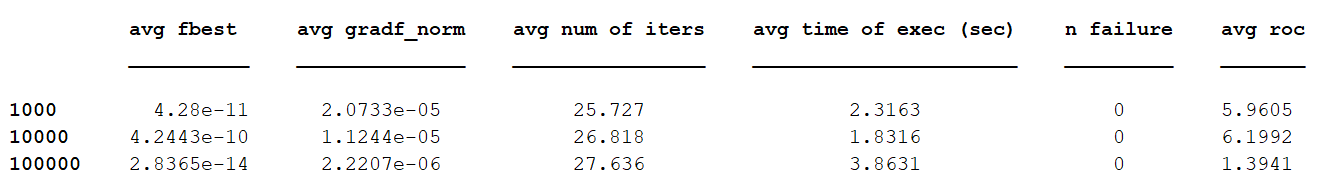
\includegraphics[width = 0.9\textwidth]{img/pb25_MN_table.png}
    \caption{Results obtained by running the Modified Newton method on the problem $25$ using the exact derivatives.}
    \label{MN25}
\end{figure*}

As expected from the theoretical background we have about these methods, the Modified Newton method performs significantly better than the Nealder Mead method. The table shows that the method converges to a point in which the norm of the gradient is below the fixed tolerance for all dimensionalities tested, and the minimum value found is consistently close to zero. 
This is because the Modified Newton method uses the gradient and Hessian information, allowing it to make more informed steps towards the minimum and thus to converge in fewer iterations.

However, we can notice that the ratio between the average time of execution and the average number of iterations is smaller for the simplex method. This means that each iteration performed by the Modified Newton method is more high-performance but also more costly in terms of computational effort. 

\medskip
\subsection*{Modified Newton Method - Approximated Derivatives}
Approximating the derivatives of the function $F(\mathbf{x})$ using finite differences is more challenging than it appears due to potential numerical cancellation issues, which can occur when subtracting two nearly equal quantities. Additionally, we aim to derive a formula that minimizes computational cost.

As done previously we will first consider the case in which the dimensionality $n$ is an even integer and then we will specify what changes if $n$ is an odd number.

Let's begin by approximating the first order derivatives by using the centered finite difference formula with increment $h_k$. We keep track of the subscript $k$ in order to derive formula which are valid both for the case with constant increments and the case in which the increments depend on the components respect to which we are differentiating.
The general formula is
$$ \frac{\partial F }{\partial x_k} (\mathbf{x}) \approx \frac{F(\mathbf{x} + h_k \vec{e}_k) - F(\mathbf{x} - h_k \vec{e}_k)}{2h_k} = 
\frac{\sum_{i = 1}^{n} f_i(\mathbf{x} + h_k \vec{e}_k)^2 - \sum_{i = 1}^{n} f_i(\mathbf{x} - h_k \vec{e}_k)^2}{4h_k}$$
but it would not be much wise to apply it directly to out problem because it would be unnecessary to evaluate all the terms $f_i^2(\mathbf{x})$ which are not affected by the variation of the $k$-th component of the vector $\mathbf{x}$.
In particular, we can notice that if we are differentiating with respect to an even component the only term we need to compute is $f_{k-1}^2()$, while if we are differentiating with respect to an odd component we only need to expand the terms $f_k^2()$ and $f_{k+1}^2()$.
Omitting the calculus, we obtain the following formula
\begin{align*}
    \frac{\partial F}{\partial x_k} (\mathbf{x}) &\approx \frac{f_{k-1}^2(\mathbf{x} + h_k \vec{e}_k) - f_{k-1}^2(\mathbf{x} - h_k \vec{e}_k)}{4h_k} = \frac{- 40h_k (10x_{k-1}^2 - 10x_k)}{4h_k} \quad  &\mod(k,2)  = 0 \\
    \frac{\partial F}{\partial x_k} (\mathbf{x}) &\approx \frac{f_{k}^2(\mathbf{x} + h_k \vec{e}_k) - f_{k}^2(\mathbf{x} - h_k \vec{e}_k) + f_{k+1}^2(\mathbf{x} + h_k \vec{e}_k) - f_{k+1}^2(\mathbf{x} - h_k \vec{e}_k)}{4h_k} \\ &= \frac{80x_k h_k (10x_k^2 + 10 h_k^2 -10x_{k+1}) - 4h_k (x_k -1)}{4h_k} \quad &\mod(k,2) = 1
\end{align*}

If $n$ is an odd number, the approximation of $\frac{\partial F}{\partial x_1} (\mathbf{x})$ will slightly change into 
\begin{align*}
\frac{\partial F}{\partial x_1} (\mathbf{x}) & \approx  \frac{f_{1}^2(\mathbf{x} + h_1 \vec{e}_1) - f_{1}^2(\mathbf{x} - h_1 \vec{e}_1) + f_{2}^2(\mathbf{x} + h_1 \vec{e}_1) - f_{2}^2(\mathbf{x} - h_1 \vec{e}_1) + f_n^2(\mathbf{x} + h_1 \vec{e}_1) - f_n^2(\mathbf{x} - h_1\vec{e}_1)}{4h_1} \\ &
 = \frac{80x_1 h_1(10x_1^2 + 10 h_1^2 -10x_{2}) - 4h_1 (x_1 -1) -40h_1 (10x_n^2 - 10x_1) }{4h_1}
\end{align*}

For what concerns the second order derivatives, we can apply a similar reasoning based on neglecting the terms $f_i^2(\mathbf{x})$ which are not affected by the variation of the $k$-th component of $\mathbf{x}$ but starting from the general formula
$$ \frac{\partial^2 F}{\partial x_i \partial x_j} (\mathbf{x})  = \frac{F(\mathbf{x} + h_i \vec{e}_i + h_j \vec{e}_j) - F(\mathbf{x} + h_i \vec{e}_i) - F(\mathbf{x} - h_j \vec{e}_j) + F(\mathbf{x})}{h_i h_j}$$
Due to the particular structure of the problem we are considering, many second order derivatives are zero, thus we are going to approximate solely the ones we know are not null.
\begin{align*}
    & \frac{\partial^2 F}{\partial x_k^2} (\mathbf{x}) \approx \frac{f_{k-1}^2 (\mathbf{x} + 2h_k \vec{e}_k) - 2 f_{k-1}^2 (\mathbf{x} + h_k \vec{e}_k) + f_{k-1}(\mathbf{x})}{2h_k^2} = \frac{200h_k^2}{2 h_k^2}, & \mod(k,2) = 0 \\
    & \frac{\partial^2 F}{\partial x_k^2} (\mathbf{x}) \approx \frac{f_{k}^2 (\mathbf{x} + 2h_k \vec{e}_k) - 2 f_{k}^2 (\mathbf{x} + h_k \vec{e}_k) + f_{k}(\mathbf{x}) + f_{k+1}^2 (\mathbf{x} + 2h_k \vec{e}_k) - 2 f_{k+1}^2 (\mathbf{x} + h_k \vec{e}_k) + f_{k+1}(\mathbf{x})}{2h_k^2} \\
    & \qquad = \frac{40h_k^2 (10x_k^2 - 10x_{k+1}) + 1400 h_k^4 + 2400h_k^3 x_k + 800 x_k h_k^2 + 2h_k^2}{2 h_k^2}, & \mod(k,2) = 1 \\
    & \frac{\partial^2 F}{\partial x_k \partial x_{k+1}} (\mathbf{x}) \approx \frac{f_{k}^2 (\mathbf{x} + h_k \vec{e}_k + h_{k+1} \vec{e}_{k+1}) - f_{k}^2 (\mathbf{x} + h_k \vec{e}_k) - f_{k}^2 (\mathbf{x} + h_{k+1} \vec{e}_{k+1}) + f_{k}(\mathbf{x})}{2h_k h_{k+1}} \\
    & \qquad = \frac{20h_{k+1} (-10h_k^2 - 20h_k x_k)}{2h_k h_{k+1}}, & \mod(k,2) = 1
\end{align*}
We explicitly approximated just the superior diagonal, the inferior one is obtained by imposing the symmetry of the hessian matrix.

If the dimensionality $n$ is an odd number, the changes only concern the term  $\frac{\partial^2 F}{\partial x_1^2} (\mathbf{x})$ and the external diagonal which are not null anymore. In particular, these terms become
\begin{align*}
    \frac{\partial^2 F}{\partial x_1^2} (\mathbf{x}) & \approx\frac{40h_1^2 (10x_1^2 - 10x_{2}) + 1400 h_1^4 + 2400h_1^3 x_1 + 800 x_1 h_1^2 + 202h_1^2 }{2 h_k1^2} \\
    \frac{\partial^2 F}{ \partial x_n \partial x_1} & = \frac{\partial^2 F}{ \partial x_1 \partial x_n} \approx \frac{20h_1(-20x_n h_n - 10h_n^2 )}{2h_1 h_n}
\end{align*}


According to what we expect, seeking for the minimum using the approximations of the derivatives affects the performance of the Modified Newton method, especially for larger values of the increment $h$. 
In fact, from the theory, we know that the finite difference formula approximates the analytical derivative with an error that depends on the value of the increment $h$. Specifically, the error diminishes as $h$ approaches $0$.

\begin{figure}[htbp]
    \centering
    % Prima immagine
    \begin{subfigure}[t]{0.45\textwidth}  % Larghezza del 45% del testo
        \centering
        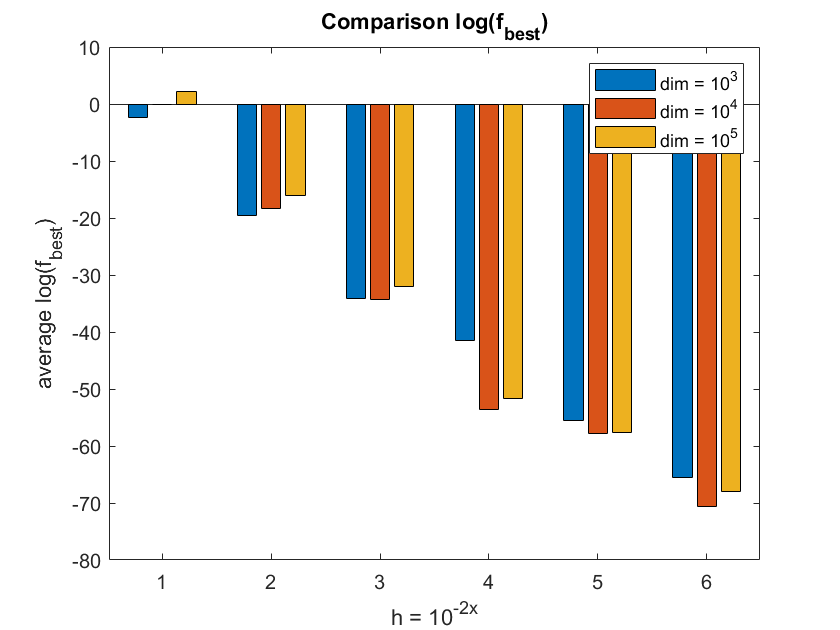
\includegraphics[width=\textwidth]{img/pb25_MN_difffinite_COST_log(fbest).png}
        \caption{Costant Increment $h$}
    \end{subfigure}
    \hspace{1cm} %spaziatura tra le immagini
    % Seconda immagine
    \begin{subfigure}[t]{0.45\textwidth}
        \centering
        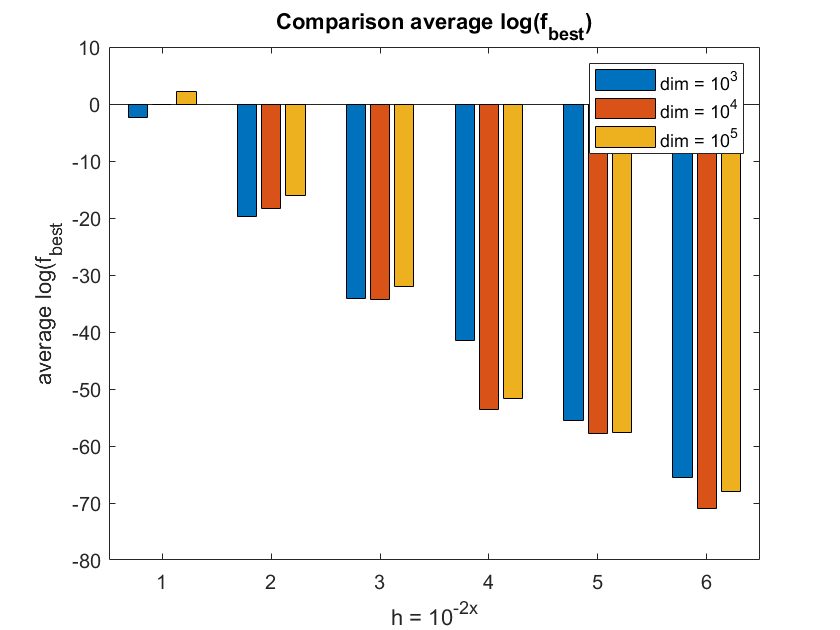
\includegraphics[width=\textwidth]{img/pb25_MN_difffinite_REL_log(fbest).png}
        \caption{Specific Increment }
    \end{subfigure}
    % Didascalia generale
    \caption{ \small Values of the average $\log(f_{best})$ in function of the increment while running the Modified Newton Method with approximated derivatives on the problem $25$.}
    \label{logfbest_difffinite25}
\end{figure}

Therefore, it is not surprising that for $h = 10^{-2}$, the algorithm often converges to a point whose value is not very close to $0$ and requires significantly more iterations to meet the stopping criterion.
This is clearly shown in the following bar plots (Figure \ref{logfbest_difffinite25}), which display the average value of $\log (f_{best})$, where $f_{best}$ is the minimum found by the Modified Newton method, as a function of the increment $h$ used to approximate the derivatives. Notice that we applied a logarithmic transformation to the value of $f_{best}$ for clarity, as the values were close to $0$.
As we can see from the barplot, as the value of $h$ diminish the minimum found is smaller (i.e. $\log(f_{best})$ increases in absolute value while being a negative quantity) as a consequence of the more precise approximations of the derivatives the Modified Newton method uses.


\begin{figure*}[htbp]
    \centering
    % Prima immagine
    \begin{subfigure}[t]{0.45\textwidth}  % Larghezza del 45% del testo
        \centering
        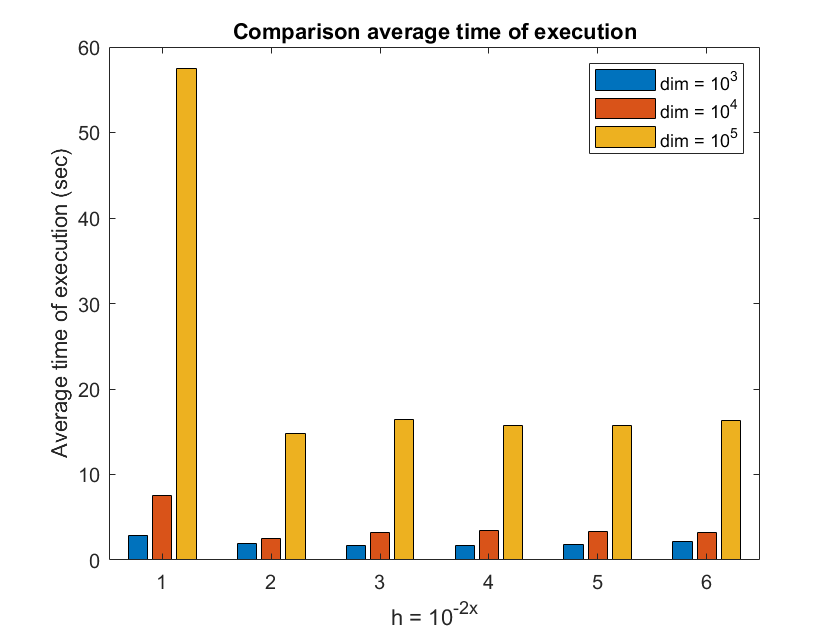
\includegraphics[width=\textwidth]{img/pb25_MN_difffinite_COST_timeofexec.png}
        \caption{Constant Increment $h$}
    \end{subfigure}
    \hspace{1cm} %spaziatura tra le immagini
    % Seconda immagine
    \begin{subfigure}[t]{0.45\textwidth}
        \centering
        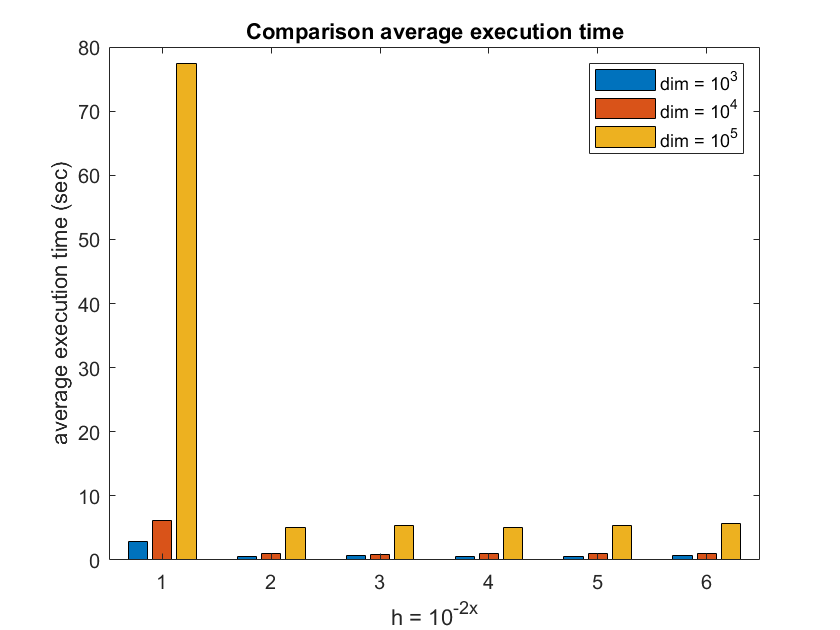
\includegraphics[width=\textwidth]{img/pb25_MN_difffinite_REL_timeofexec.png}
        \caption{Specific Increment }
    \end{subfigure}
    % Didascalia generale
    \caption{ \small Average time of execution in function of the increment $h$  while running the Modified Newton Method with approximated derivatives on the problem $25$.}
\end{figure*}

\begin{figure}[htbp]
    \centering
    % Prima immagine
    \begin{subfigure}[t]{0.45\textwidth}  % Larghezza del 45% del testo
        \centering
        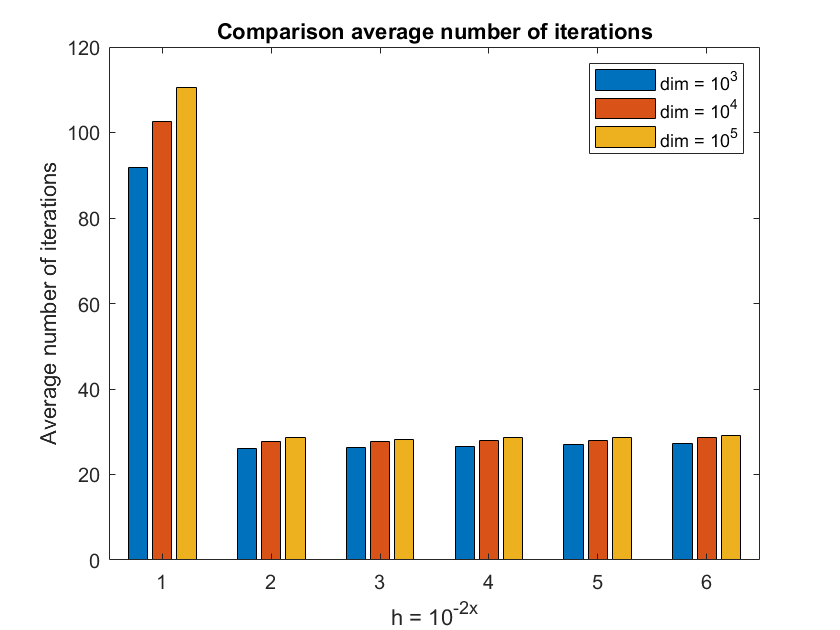
\includegraphics[width=\textwidth]{img/pb25_MN_difffinite_COST_avgiterations.png}
        \caption{Constant Increment $h$}
    \end{subfigure}
    \hspace{1cm} %spaziatura tra le immagini
    % Seconda immagine
    \begin{subfigure}[t]{0.45\textwidth}
        \centering
        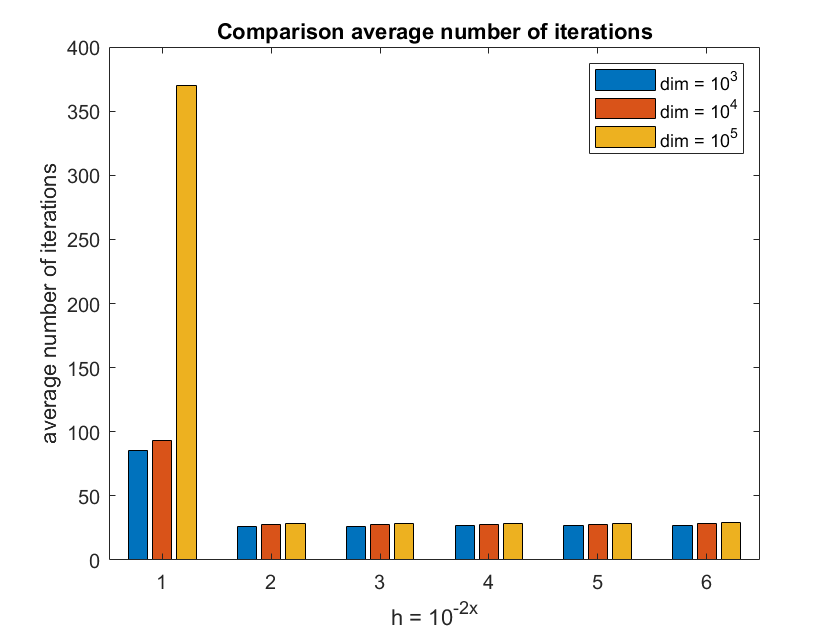
\includegraphics[width=\textwidth]{img/pb25_MN_difffinite_REL_avgiterations.png}
        \caption{Specific Increment}
    \end{subfigure}
    % Didascalia generale
    \caption{ \small Average number of iterations in function of the increment $h$  while running the Modified Newton Method with approximated derivatives on the problem $25$.}
    \label{avgiterations25}
\end{figure}


\begin{figure*}[htbp]
    \centering
    % Prima immagine
    \begin{subfigure}[t]{0.45\textwidth}  % Larghezza del 45% del testo
        \centering
        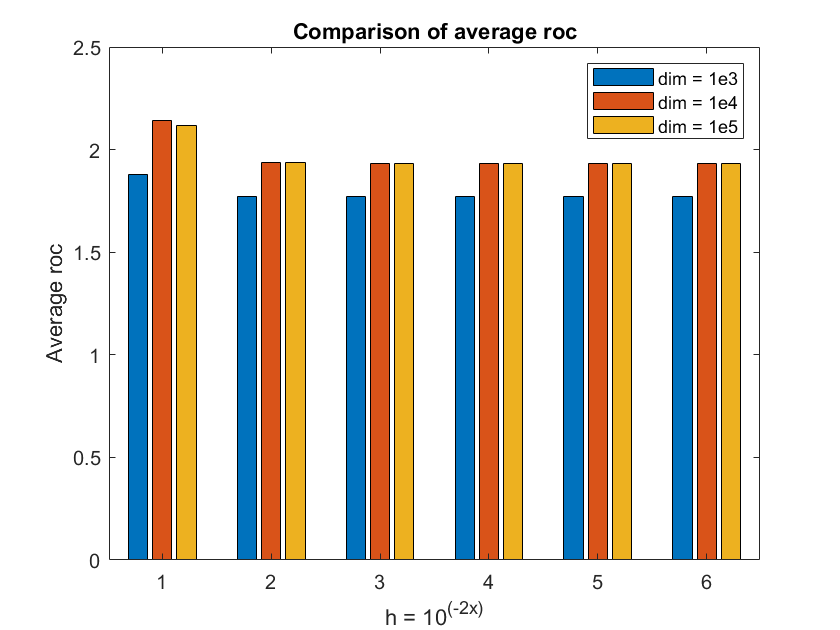
\includegraphics[width=\textwidth]{img/pb76_MN_difffinite_COST_rateofconv.png}
        \caption{Constant Increment $h$}
    \end{subfigure}
    \hspace{1cm} %spaziatura tra le immagini
    % Seconda immagine
    \begin{subfigure}[t]{0.45\textwidth}
        \centering
        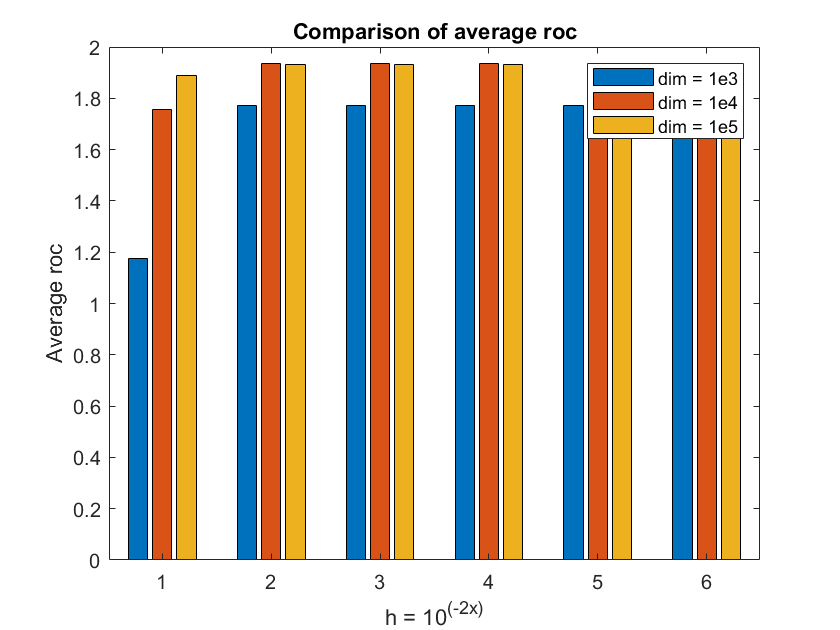
\includegraphics[width=\textwidth]{img/pb76_MN_difffinite_REL_rateofconv.png}
        \caption{Specific Increment }
    \end{subfigure}
    % Didascalia generale
    \caption{ \small Average values of the experimental rate of convergence in function of the increment $h$  while running the Modified Newton Method with approximated derivatives on the problem $25$.}
    \label{25roc}
\end{figure*}


It can be interesting notice from the barplots comparing the average number of iterations needed by the Modified Newton method (Figure $\eqref{avgiterations25}$) that a specific increment based on the point in which we are approximating the derivative seems to make the method perform better than using the constant increment.  

Lastly we can also notice that the average rate of convergence, shown in the barplots $\eqref(25roc)$, is still close to the expected value $2$ and it is on average higher when the increment is constant for each component of the point in which we are approximating the derivatives.
This means that all the efforts we put in to avoid numerical cancellation and to derive a more efficient formula for the finite differences have paid off. The results show that the Modified Newton method with approximated derivatives can still achieve a good performance, especially when using a specific increment based on the point in which we are approximating the derivative. 